\documentclass[twoside,11pt]{article}
\usepackage[left=1in, right=1in, top=1in, bottom=1in]{geometry}
\usepackage{amsmath}
\usepackage{amssymb}
\usepackage{amsfonts}
\usepackage{mathtools}
\usepackage{amsthm}
\usepackage{fancyhdr}
\usepackage{enumitem}
\usepackage{siunitx}
\usepackage{booktabs}
\usepackage[hidelinks]{hyperref}
\usepackage{sectsty}
\usepackage{mathrsfs} % mathscr
\usepackage{tikz}
\usepackage{pgfplots}
\usepackage{multicol}
\usepackage{listings}
% \usepackage{amsart}
\usepackage{fontspec}
\usepackage{soul}


% allow H option of figure
\usepackage{float}

% math font (libertine)
\usepackage{libertinus-otf}

% braket
\usepackage{braket}

% tikz library
\usetikzlibrary{decorations,calligraphy,calc,external}
\tikzexternalize
\tikzexternaldisable

% physics
% \usepackage{physics}

% define latin modern font environment
\newcommand{\lms}{\fontfamily{lmss}\selectfont} % Latin Modern Roman
% \newcommand{\lmss}{\fontfamily{lmss}\selectfont} % Latin Modern Sans
% \newcommand{\lmss}{\fontfamily{lmtt}\selectfont} % Latin Modern Mono

% % change mathcal shape
% \usepackage[mathcal]{eucal}


% define math operators
\newcommand{\FF}{\mathbb{F}}
\newcommand{\RR}{\mathbb{R}}
\newcommand{\NN}{\mathbb{N}}
\newcommand{\ZZ}{\mathbb{Z}}
\newcommand{\QQ}{\mathbb{Q}}
\newcommand{\XX}{\mathbb{Y}}
\newcommand{\CL}{\mathcal{L}}
% \renewcommand{\d}{\mathrm{d}}
\renewcommand*\d{\mathop{}\!\mathrm{d}}
\DeclareMathOperator*{\argmax}{arg\,max}
\DeclareMathOperator*{\argmin}{arg\,min}
\DeclareMathOperator{\im}{im}
\DeclareMathOperator{\id}{id}
\DeclareMathOperator{\erf}{erf}
\renewcommand{\mod}[1]{\ (\mathrm{mod}\ #1)}

% section font style
\sectionfont{\sffamily\Large}
\subsectionfont{\sffamily\normalsize}
\subsubsectionfont{\bf}

% line spreading and break
\hyphenpenalty=5000
\tolerance=20
\setlength{\parindent}{0em}
\setlength\parskip{0.5em}
\allowdisplaybreaks
\linespread{0.9}

% enumerate settings
% no break before enumerate
\setlist[enumerate]{itemsep=2pt,topsep=2pt}

% theorem
% latex theorem
% definition style
\theoremstyle{definition}
\newtheorem{theorem}{\lms Theorem}[subsection]
\newtheorem{axiom}{\lms Axiom}[section]
\newtheorem{definition}{\lms Definition}[section]
\newtheorem{example}{\lms Example}[section]
\newtheorem{question}{\lms Question}[section]
\newtheorem{exercise}{\lms Exercise}[section]
\newtheorem*{exercise*}{\lms Exercise}
\newtheorem{lemma}{\lms Lemma}[section]
\newtheorem{proposition}{\lms Proposition}[section]
\newtheorem{corollary}{\lms Corollary}[section]
\newtheorem*{theorem*}{\lms Theorem}
\newtheorem{problem}{\lms Problem}
% remark style
\theoremstyle{remark}
\newtheorem*{remark}{\lms Remark}
\newtheorem*{solution}{\lms Solution}
\newtheorem*{claim}{\lms Claim}


% paragraph indent
\setlength{\parindent}{0em}
\setlength\parskip{0.5em}

\newcommand\Code{PHY3110 SP23}
\newcommand\Ass{HW04}
\newcommand\name{Haoran Sun}
\newcommand\mail{haoransun@link.cuhk.edu.cn}

\title{{\lms \Code \ \Ass}}
\author{\lms \name \ (\href{mailto:\mail}{\mail})}
\date{\sffamily \today}

\makeatletter
% \let\Title\@title
\let\theauthor\@author
\let\thedate\@date

\fancypagestyle{plain}{%
    \fancyhf{}
    \lhead{\lms \Ass}
    \rhead{\lms \name}
    \rfoot{\lms\thepage}

    % # 页脚自定义
    \fancyfoot[L]{
        \begin{minipage}[c]{0.06\textwidth}
            \includegraphics[height=7.5mm]{logo2.png}
        \end{minipage}
    }
}
\fancypagestyle{title}{%
    \fancyhf{}
    \renewcommand{\headrulewidth}{0pt}
    % \lhead{\Title}
    % \rhead{\theauthor}
    \rfoot{\lms\thepage}

    % # 页脚自定义
    \fancyfoot[L]{
        \begin{minipage}[c]{0.06\textwidth}
            \includegraphics[height=7.5mm]{logo2.png}
        \end{minipage}
    }
}
\fancyfootoffset[L]{0.3cm}

% re-define title format
\makeatletter
\renewcommand{\maketitle}{\bgroup\setlength{\parindent}{0pt}
\begin{flushleft}
  \textbf{\Large\@title}

  \@author
\end{flushleft}\egroup
}
\makeatother

\pagestyle{plain}

% lstlisting settings
\lstset{
    basicstyle=\linespread{0.7}\footnotesize,
    breaklines=true,
    basewidth=0.5em
}


\begin{document}
\maketitle
\thispagestyle{title}
% \begin{multicols*}{2}

% \begin{remark}
%     $V_\epsilon(x)$ is used to denote a $\epsilon$-neighborhood
%     \begin{align*}
%         V_\epsilon(x) = B_\epsilon(x)\setminus\{x\}
%     \end{align*}
% \end{remark}

\begin{problem}
Use the EOM for a point mass m moving in a central potential
$V (r)$, show that ($u = 1/r$, $l$ is the angular momentum)
\begin{align*}
    \frac{\d^2 u}{\d \theta^2} + u &= -\frac{m}{l^2}\frac{\d }{\d u} V(1/u)
\end{align*}
\end{problem}
\begin{solution}
The EOM write
\begin{align*}
    m\ddot r - \frac{l^2}{mr^3} + \frac{\d}{\d r} V &= 0\\
    \dot{\theta} &= \frac{l}{mr^2}
\end{align*}
Note that
\begin{align*}
    \dot\theta &= 
    \frac{l}{mr^2} \Rightarrow
    \frac{\d}{\d t} = 
    \frac{l}{mr^2}\frac{\d}{\d\theta}
\end{align*}
Let $u=1/r$, then
\begin{align*}
    \dot r &= \frac{l}{m}u^2\frac{\d}{\d\theta}\frac{1}{u} = -\frac{l}{m}\frac{\d u}{\d \theta},\quad
    \ddot r = -\frac{l^2}{m^2} u^2\frac{\d^2 u }{\d\theta^2}
\end{align*}
Then we have
\begin{align*}
    -\frac{l^2}{m}u^2\frac{\d^2 u}{\d\theta^2} - \frac{l^2}{m}u^3 - u^2\frac{\d}{\d u}V &= 0\\
    \Rightarrow
    \frac{\d^2 u}{\d \theta^2} + u &= -\frac{m}{l^2}\frac{\d }{\d u} V
\end{align*}
\end{solution}


\begin{problem}
If the orbit of a point mass under a central force $F(r)$ is given by $r = k\theta^2$ with
$k$ being a constant, try to derive the explicit form of $F(r)$.
\end{problem}
\begin{solution}
Note that we have $r=k\theta^2$, and since $\dot\theta = l/(mr^2) = l/(mk^2r^4)$, then
\begin{align*}
    \dot r &= 
    \frac{\d}{\d t}k\theta^2 = \frac{l}{mk^2}\theta^{-4}\frac{\d}{\d\theta}k\theta^2
    = \frac{2l}{mk}\theta^{-3}\\
    \ddot r &=\cdots = -\frac{6l^2}{m^2k^3}\theta^{-8}
\end{align*}
which means
\begin{align*}
    m\ddot r - \frac{l^2}{mr^3} + \frac{\d}{\d r}V &= 0
    \Rightarrow
    F(r) = -\frac{\d}{\d r}V = -\frac{6kl^2}{m}r^{-4} - \frac{l^2}{m}r^{-3}
\end{align*}
\end{solution}


\begin{problem}
Two particles move around each other in circular orbits under gravitational
forces with a period $\tau$. If they suddenly stop at a given instant and then start to fall into each
other, show that they collide after a time $\tau/(4\sqrt{2})$.
\end{problem}
\begin{solution}
Let $m$ denotes the reduced mass and $l$ denotes the angular momentum.
Since for the circular orbits with $r=r_0$, 
the energy equals to the minimum of effective potential, which means
\begin{align*}
    \left. \frac{\partial V_\text{eff}}{\partial r} \right|_{r=r_0}
    &= 0
    \Rightarrow 
    r_0 = \frac{l^2}{mk}
\end{align*}
Then we can solve $\dot\theta$ (which is a constant) and $\tau$
\begin{align*}
    \dot\theta &= 
    \frac{l}{mr_0^2} = \frac{mk^2}{l^3},\quad
    \tau = \frac{2\pi}{\dot\theta}
    = \frac{2\pi l^3}{mk^2}
\end{align*}

Suppose two particles suddenly lose velocity at $r=r_0$,
then the angular momentum of the system vanishes.
Hence
\begin{align*}
    E &= \frac{1}{2}m\dot{r}^2 - \frac{k}{r} = -\frac{k}{r_0}
    \Rightarrow
    \dot{r} = -\left[
        \frac{2k}{m}\left(
            \frac{1}{r} - \frac{1}{r_0}
        \right)
    \right]^{1/2}
\end{align*}
To calculate the time when two particles collide, simply integrate the equation
\begin{align*}
    \dot{r} &= -\left[
        \frac{2k}{m}\left(
            \frac{1}{r} - \frac{1}{r_0}
        \right)
    \right]^{1/2}\\
    \d t &=
    -\left[
        \frac{2k}{m}\left(
            \frac{1}{r} - \frac{1}{r_0}
        \right)
    \right]^{-1/2}\d r\\
    \int_0^{\tau'} \d t &= 
    \int_{r_0}^0 -\left[
        \frac{2k}{m}\left(
            \frac{1}{r} - \frac{1}{r_0}
        \right)
    \right]^{-1/2}\d r
\end{align*}
Since
\begin{align*}
    \int_0^a\left(\frac{1}{x} - a\right)^{-1/2}\d x  
    &= \int_{1/a}^\infty \left(u - a\right)^{-1/2}\d\frac{1}{u}\\
    &= \int_{1/a}^\infty\frac{1}{u^2\sqrt{u - a}}\d u\\
    &= \int_0^\infty\frac{1}{(v^2+a)^2 v}\d (v^2 + a)\\
    &= \int_0^\infty \frac{2}{(v^2+a)^2}\d v\\
    &= \left.\frac{1}{a}\frac{v}{v^2 + a} + \frac{1}{a^{3/2}}\arctan\frac{v}{\sqrt{a}}\right|_{v=0}^{v=\infty}
\end{align*}
Hence we have the expression of $\tau'$ and 
we can prove its relationship with $\tau$
\begin{align*}
    \tau' &= 
    \left(\frac{2k}{m}\right)^{-1/2}
    \left[
        r_0\frac{v}{v^2 + 1/r_0} + r_0^{3/2}\arctan\sqrt{r_0} v
    \right]_{v=0}^{v=\infty}\\
    &= 
    \left(\frac{2k}{m}\right)^{-1/2}
    r_0^{3/2}\frac{\pi}{2}\\
    &= \left(\frac{m}{k}\right)^{1/2}
    \left(\frac{l^2}{mk^2}\right)^{3/2}\frac{\pi}{2\sqrt{2}}\\
    &= \frac{l^3}{mk^2}\frac{\pi}{2\sqrt{2}}\\
    &= \frac{\tau}{4\sqrt{2}}
\end{align*}
\end{solution}


\begin{problem}
A particle moves in a force field described by
\begin{align*}
    V(r) &= -k\frac{e^{-ar}}{r}
\end{align*}
where $k$, $a$ are positive constants
\begin{enumerate}[label=\alph*)]
    \item Use the effective potential to discuss the qualitative nature of the orbits for different values
    of energy and angular momentum.
    \item What is the period of the motion when the orbit is a circle?
\end{enumerate}
\end{problem}
\begin{solution}~
\begin{enumerate}[label=\alph*)]
\item The effective potential and its first derivative writes
\begin{align*}
    V_\text{eff} &= 
    -k\frac{e^{-ar}}{r} + \frac{l^2}{2m}\frac{1}{r}\\
    \frac{\d }{\d r} V_\text{eff} &=
    \frac{1}{r^3}\left(akr^2e^{-ar} + kre^{-ar} - \frac{l^2}{m}\right)
\end{align*}
Investigating into $f(r) = akr^2 e^{-ar} + kre^{-ar}-l^2/m$,
we have $f'(r) = e^{-ar}(-a^2kr^2 + 2akr + k)$.
This means $f(r)$ is first monotonically increasing and then decreasing,
and $f(r)$ only have one extreme value.
Regarding the sign of $f(r)$, there are only two cases
\begin{figure}[H]
    \centering
    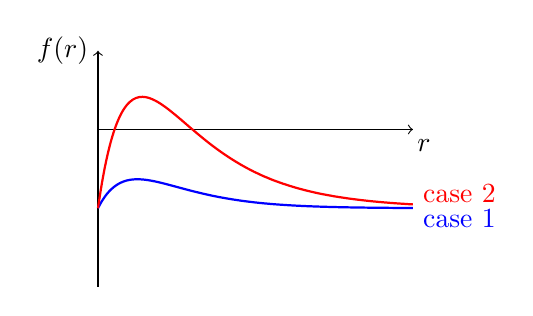
\begin{tikzpicture}
        \draw[->] (0, 0) -- (4, 0) node[below,xshift=4pt] {$r$};
        \draw[->] (0, -2) -- (0, 1) node[left] {$f(r)$};
        \draw[thick,domain=0:4,variable=\x,smooth,samples=100,blue]
            plot ({\x}, {2*\x*exp(-2*\x) - 1})
            node[right,yshift=-4pt] {case 1};
        \draw[thick,domain=0:4,variable=\x,smooth,samples=100,red]
            plot ({\x}, {7*\x*exp(-2*\x) + \x^2 * exp(-1.5*\x) - 1})
            node[right,yshift=4pt] {case 2};
    \end{tikzpicture}
\end{figure}
Since $f(r)$ shares the same sign with $V_\text{eff}$,
we also have two cases for $V_\text{eff}$ 
\begin{enumerate}[label=\roman*.]
\item $V_\text{eff}$ is always decreasing, there are no bounded solutions.

\item $V_\text{eff}$ looks like the following figure
\begin{figure}[H]
    \centering
    \begin{tikzpicture}
        \draw[->] (0, 0) -- (7, 0) node[below,xshift=4pt] {$r$};
        \draw[->] (0, -2) -- (0, 3) node[left] {$V_\text{eff}$};
        \draw[thick,domain=0.46:6.8,variable=\x,smooth,samples=200]
            plot ({\x}, {20 * (1/(2*\x^2) - 1.86 * exp(-1.3*\x) / \x)});
        \draw[dashed] (0.699, -0.983) -- (0.699, 0) node[above] {$r_0$} 
                                                    node[circle,fill,inner sep=1pt] {};
        \draw[dashed] (1.988, 1.119)  -- (1.988, 0) node[below] {$r_1$}
                                                    node[circle,fill,inner sep=1pt] {};
    \end{tikzpicture}
\end{figure}
\end{enumerate}
Hence, $V_\text{eff}$ will have a local minimum at $r_0$ 
and a local maximum at $r_1$.
The solution will be bounded if $E < V_\text{eff}(r_1)$.

\item The circular motion is only possible for the case ii.
Hence we have $f(r_1) = f(r_2) = 0$, then we can solve $\dot\theta$ and $\tau$
(where $r^*$ is either $r_1$ or $r_2$)
\begin{align*}
    l^2 &= mkr(1+ar)e^{-ar}
    \Rightarrow\dot\theta = \frac{l}{m{r^*}^2} = 
    \left[\frac{k(1+ar)}{m{r^*}^3}\right]^{1/2}e^{-a{r^*}/2}
    ,~
    \tau = \frac{2\pi}{\dot\theta} = 
    2\pi\left[\frac{m{r^*}^3}{k(1+a{r^*})}\right]^{1/2}e^{a{r^*}/2}
\end{align*}
\end{enumerate}
\end{solution}




% \end{multicols*}
\end{document}

